%%%%%%%%%%%%%%%%%%%%%%%%%%%%%%%%%%%%%%%%%%%%%%%%%%%%%%%%%%%%%%%%%%%%%%%%%%%

\documentclass{standalone}

\usepackage{amsmath}
\usepackage{mathptmx}
\usepackage{pgfplots}
\usetikzlibrary{external}
\tikzexternalize{coin-flip-scatterplot}
\pgfplotsset{compat=1.15}

%% IEEE uses Times Roman font, so we'll default to Times.
%% These three commands make up the entire times.sty package.
\renewcommand{\rmdefault}{ptm}
\renewcommand{\ttdefault}{pcr}
\normalfont\selectfont

\begin{document}

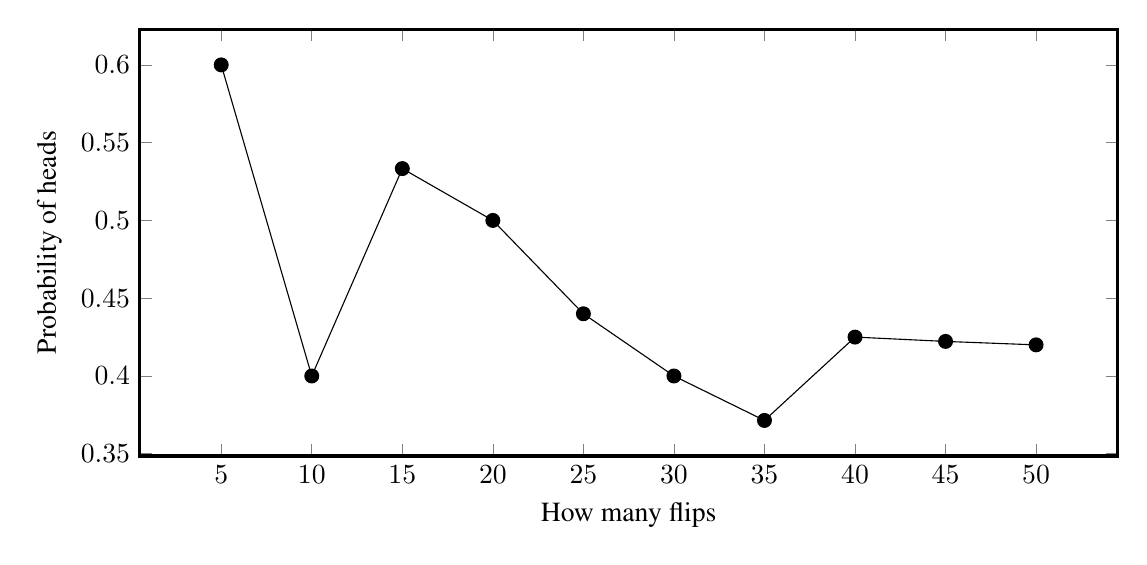
\begin{tikzpicture}
\tikzset{%%
  every mark/.append style={scale=1.0},%%
  scale=1.0%%
}
\pgfplotsset{%%
  every axis/.append style={font=\normalsize}%%
}
%%
\begin{axis}[%%
  axis line style=very thick,%%
  dotStyle/.style={mark size=2.5,black,mark color=black,mark=*},%%
  enlargelimits=true,%%
  height=7cm,%%
  plotStyle/.style={%%
    domain=4:17,%%
    mark=none,%%
    smooth,%%
    thick%%
  },%%
  width=14cm,%%
  xlabel={\normalsize How many flips},%%
  ylabel={\normalsize Probability of heads}%%
]
%%
%%
\addplot[dotStyle] coordinates {
  (5, 0.6)
  (10, 0.4)
  (15, 0.533333333333333)
  (20, 0.5)
  (25, 0.44)
  (30, 0.4)
  (35, 0.371428571428571)
  (40, 0.425)
  (45, 0.422222222222222)
  (50, 0.42)
};
\end{axis}
\end{tikzpicture}

\end{document}
